\documentclass[12pt]{report}
\usepackage[utf8]{inputenc}
\usepackage{graphicx}
\usepackage[a4paper,width=150mm,top=25mm,bottom=25mm]{geometry}
\usepackage{pgfplots}
\usepackage{mathtools,amssymb}
\usepackage{tikz}
\usepackage{xcolor}
\usepackage[backend=biber,style=numeric,sorting=ynt]{biblatex}
\usepackage{hyperref}
\usepackage{indentfirst}

\hypersetup{
    colorlinks=true,
    linkcolor=black,
    filecolor=magenta,      
    urlcolor=blue,
    citecolor=blue,
    pdftitle={Pthreads and openCilk systems},
}

\pgfplotsset{compat=1.7}
\graphicspath{ {images/} }
\addbibresource{bib/bibliography.bib}


\begin{document}

    \author{Vasilis Kyriafinis \\ email: \href{mailto:vakyriaf@ece.auth.gr}{vakyriaf@ece.auth.gr}} 

\makeatletter
\begin{titlepage}
    \begin{center}
        \vspace*{4cm}
 
        \textbf{\Large{Pthreads and openCilk models}}
 
        \vspace{0.5cm}
        \large{A comparison of the two parallel programming frameworks}
             
        \vspace{1cm}
 
        \textbf{Vasilis Kyriafinis, 9797}
 
        \vfill
                                
        Aristotle University Of Thessaloniki\\
        Parallel and Distributed Systems\\
        October 2022
        \vspace*{0cm}
             
    \end{center}
\end{titlepage}
    
    \tableofcontents
    \clearpage
    
    \addcontentsline{toc}{section}{Introduction}
    \section*{Introduction}
    \subsubsection{Assignment description}
The main point of focus of this project is to compare the pthreads and openCilk multi-threading systems through a real life application.
The main points of comparison are functionality, ease of use and performance, of the two multi-threading systems. The project uses C++ in
order to be compatible with the uint256\_t library but it is developed using structured programming logic.

\subsubsection{The real life problem}
The problem used for this comparison is file compression using the Huffman algorithm. The Huffman algorithm is a lossless data compression algorithm. 
It is a variable length code algorithm, meaning that the length of the code is not fixed. The algorithm is based on the frequency of the characters in
the file. The more frequent a character is, the shorter the code for that character will be. The algorithm performs best when the distributions of the 
frequencies is not uniform. For this reason the best compression is achieved on text files with natural language. 

The natural language uses only part of the 8bit ASCII code. A typical frequency distribution of the characters in a text file is shown in the figure below.

\begin{center}
    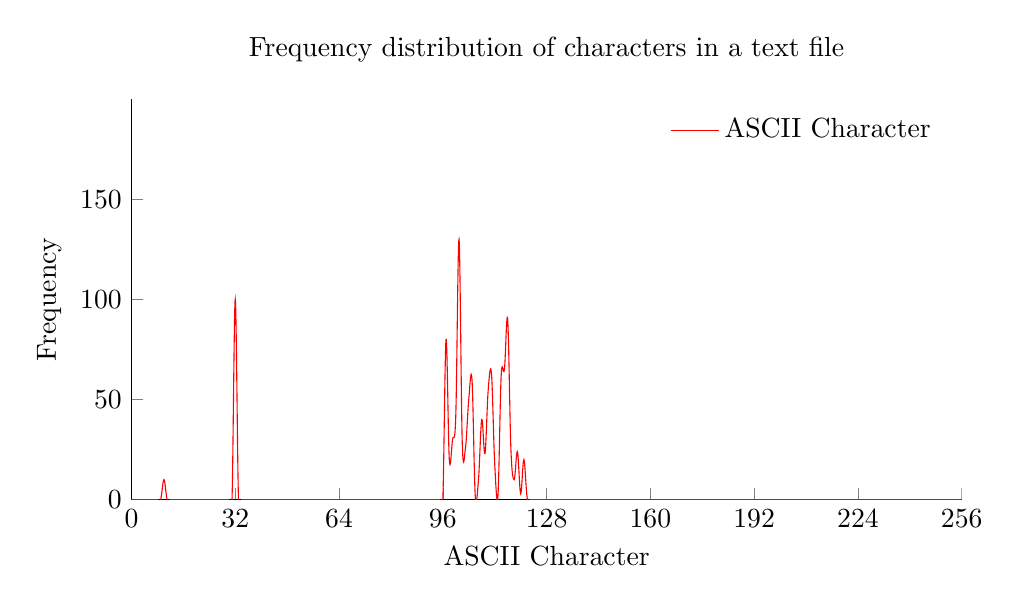
\begin{tikzpicture}
        \begin{axis}[
            title style={anchor=north,yshift=20},
            title={Frequency distribution of characters in a text file},
            axis y line*=left,
            axis x line*=bottom,
            ylabel={Frequency},
            xlabel={ASCII Character},
            ymin=0, ymax=200,
            xmin=0, xmax=256,
            xtick={0,32,64,96,128,160,192,224,256},
            ytick={0,50,100,150},
            width = \textwidth,
            height = 0.55\textwidth,
            legend style={draw=none},
        ]
        
        \addplot[
            smooth,
            tension=0.6,
            color = red,
            ]
            coordinates {
            (0,0)(1,0)(2,0)(3,0)(4,0)(5,0)(6,0)(7,0)(8,0)(9,0)(10,10)(11,0)(12,0)(13,0)(14,0)(15,0)(16,0)(17,0)(18,0)(19,0)(20,0)(21,0)(22,0)(23,0)(24,0)(25,0)(26,0)(27,0)
            (28,0)(29,0)(30,0)(31,0)(32,100)(33,0)(34,0)(35,0)(36,0)(37,0)(38,0)(39,0)(40,0)(41,0)(42,0)(43,0)(44,0)(45,0)(46,0)(47,0)(48,0)(49,0)(50,0)(51,0)(52,0)(53,0)(54,0)
            (55,0)(56,0)(57,0)(58,0)(59,0)(60,0)(61,0)(62,0)(63,0)(64,0)(65,0)(66,0)(67,0)(68,0)(69,0)(70,0)(71,0)(72,0)(73,0)(74,0)(75,0)(76,0)(77,0)(78,0)(79,0)(80,0)(81,0)
            (82,0)(83,0)(84,0)(85,0)(86,0)(87,0)(88,0)(89,0)(90,0)(91,0)(92,0)(93,0)(94,0)(95,0)(96,0)(97,80)(98,20)(99,30)(100,42)(101,130)(102,28)(103,26)(104,50)(105,60)
            (106,2)(107,10)(108,40)(109,23)(110,55)(111,63)(112,18)(113,2)(114,62)(115,65)(116,90)(117,25)(118,10)(119,24)(120,3)(121,20)(122,1)(123,0)(124,0)(125,0)(126,0)(127,0)(128,0)(129,0)(130,0)
            (131,0)(132,0)(133,0)(134,0)(135,0)(136,0)(137,0)(138,0)(139,0)(140,0)(141,0)(142,0)(143,0)(144,0)(145,0)(146,0)(147,0)(148,0)(149,0)(150,0)(151,0)(152,0)(153,0)
            (154,0)(155,0)(156,0)(157,0)(158,0)(159,0)(160,0)(161,0)(162,0)(163,0)(164,0)(165,0)(166,0)(167,0)(168,0)(169,0)(170,0)(171,0)(172,0)(173,0)(174,0)(175,0)(176,0)
            (177,0)(178,0)(179,0)(180,0)(181,0)(182,0)(183,0)(184,0)(185,0)(186,0)(187,0)(188,0)(189,0)(190,0)(191,0)(192,0)(193,0)(194,0)(195,0)(196,0)(197,0)(198,0)(199,0)
            (200,0)(201,0)(202,0)(203,0)(204,0)(205,0)(206,0)(207,0)(208,0)(209,0)(210,0)(211,0)(212,0)(213,0)(214,0)(215,0)(216,0)(217,0)(218,0)(219,0)(220,0)(221,0)(222,0)
            (223,0)(224,0)(225,0)(226,0)(227,0)(228,0)(229,0)(230,0)(231,0)(232,0)(233,0)(234,0)(235,0)(236,0)(237,0)(238,0)(239,0)(240,0)(241,0)(242,0)(243,0)(244,0)(245,0)
            (246,0)(247,0)(248,0)(249,0)(250,0)(251,0)(252,0)(253,0)(254,0)(255,0)(256,0)
            };
            \legend{ASCII Character}
            
        \end{axis}
    \end{tikzpicture}
\end{center}

It is clear that the most frequent characters are the letters of the alphabet. Using the Huffman coding the symbols for the most frequent characters are less than the 
original 8bits of the ASCII code. Replacing the characters with those symbols will result in a smaller file size.

\subsubsection{Huffman coding significance}

The huffman algorithm is widely used in all the mainstream compression formats. It is especially effective in the compression of images, text and audio files. It provides
lossless compression, meaning that the original file can be reconstructed from the compressed file. These reasons have lead in the widespread use of the huffman algorithm.
Because Huffman algorithm is a core element of many compression algorithms, speeding it up is very desirable, as many application will benefit from it. 


    \addcontentsline{toc}{section}{State of the Art}
    \section*{State of the Art}
    \subsubsection*{Previous papers}

Regarding the main focus point of this assignment there are plenty of papers comparing the performance of different threading programming
models. Scott R. Taylor et al. \cite{multithreading-comparison} compared the performance of cilk, pthreads and Java threads. Their approach
was to parallelize the fibonacci algorithm and to compare the performance of the different threading models. Their methodology was a time
comparison between the three different models. They found that the cilk model was the fastest one and the Java threads model was the slowest one.

On a more comprehensive level, Ensar Ajkunic et al. \cite{5-parallel-models} compared the performance of five different parallel programming models.
Pthread, OpenMP, Threading Building Blocks, Cilk++ and MPI. Their approach was similar to the one of Taylor et al. \cite{multithreading-comparison}
They compared the execution time of the algorithm written in the 5 models. The key difference was that they used matrix multiplication as the 
benchmarking algorithm. Their results also included speed up trends compared to the sequential implementation. 

At last but not least Solmaz Salehian et al. \cite{threading-models} compared the performance of multiple threading models using multiple algorithms.
The methodology was slightly different from the previous two papers. Along with the execution time they also compared the ability of the models to
scale on multiple cores and the performance gains from using more physical cores.

    \addcontentsline{toc}{section}{Objective and Methodology}
    \section*{Objective and Methodology}
    \subsubsection*{Objective}

The main focus of this assignment is to compare the pthreads and openCilk models on multiple aspects. The most important is the performance of the benchmarking
algorithm. The algorithm used as mentioned before is Huffman encoding. The sequential version of the algorithm was coded from scratch and can be found on the
accompanying Github repository along with the parallel implementations.

\subsubsection*{Methodology}
All of the test will be performed on the Ryzen 7 5700G, which is an 8 core 16 thread CPU. The variables of the tests will be the number of threads used and the size of the input file.
All other variables are kept constant in a way that other components, such as disk read and write speeds, don't interfere with the results. The input file will be
a text file containing \href{https://loremipsum.io/}{lorem ipsum } which produces character frequency distribution as shown in the introduction of this document.
The results will include an absolute time comparison and a speed up trend compared to the sequential implementation.

\subsubsection*{Key differentiation}
The main differentiation of this assignment for the previous papers is that it will also compare the ease of use of the two models as well as the functionality
the two frameworks provide. Those aspects are inherently subjective and will be discussed in the results section.

    \addcontentsline{toc}{section}{Results}
    \section*{Results}
    The results of the test run are presented bellow. Every test was averaged on multiple runs to reduce
the variance of the results and to avoid the cold cache phenomenon.

\subsubsection*{Fixed input size}

The first test run is with a fixed input size file of 2.2GB. The variable of this test is the number of threads opened by the program.
The pthread implementation is slightly faster and the best performance is achieved for 16 threads.
For more than 16 threads the performance is slowly dropping.

\begin{center}
    \begin{tikzpicture}
        \begin{axis}[
            title style={at={(0.5,0)},anchor=north,yshift=-45pt},
            title = {Time vs N. Threads for 2.2GB  input},
            axis y line*=left,
            axis x line*=bottom,
            ylabel={$Time\ (s)$},
            xlabel={N. Threads},
            ymin=0, ymax=80,
            xmin=0, xmax=24,
            xtick={0, 4, 8, 12, 16, 20, 24},
            ytick={10, 20, 30, 40, 50, 60, 70, 80},
            width = \textwidth,
            height = 0.55\textwidth,
            legend style={draw=none}
        ]
        \addplot[
            smooth,
            tension=0.1,
            color=red
        ] table [x=x, y=y] {data/pthread/time_ncores.txt};
        \addlegendentry{Pthreads}

        \addplot[
            smooth,
            tension=0.1,
            color=blue
        ] table [x=x, y=y] {data/cilk/time_ncores.txt};
        \addlegendentry{openCilk}
        \addlegendimage{empty legend}
        \addlegendentry{Sequential time 150s}
        % \legend{Pthreads, openCilk}
        \end{axis}
        \end{tikzpicture}
\end{center}

\subsubsection*{Fixed number of threads}

The testing methodology is the same with the previous test, but this time the number of threads is
fixed to 16. The variable for this test is the size of the input file. From the graph bellow, it can
be seen that both models scale linearly with the input size and the performance is almost the same.

\begin{center}
    \begin{tikzpicture}
        \begin{axis}[
            title style={at={(0.5,0)},anchor=north,yshift=-45pt},
            title = {Time vs File size for 16 threads},
            axis y line*=left,
            axis x line*=bottom,
            ylabel={$Time\ (s)$},
            xlabel={$File\ size\ (MB)$},
            ymin=0, ymax=20,
            xmin=0, xmax=2500,
            ytick={0, 4, 8, 12, 16, 20},
            xtick={500, 1000, 1500, 2000, 2500},
            width = \textwidth,
            height = 0.55\textwidth,
            legend style={draw=none}
        ]
        \addplot[
            smooth,
            tension=0.1,
            color=red
        ] table [x=x, y=y] {data/pthread/time_inputsize.txt};
        \addlegendentry{Pthreads}

        \addplot[
            smooth,
            tension=0.1,
            color=blue
        ] table [x=x, y=y] {data/cilk/time_inputsize.txt};
        
        \addlegendentry{openCilk}
        \addlegendimage{empty legend}
        \end{axis}
        \end{tikzpicture}
\end{center}

This behavior is also present in the sequential algorithm, with the only difference being the execution
time. This shows that both of the parallel implementations have the same time complexity with regard to 
the input size.


\begin{center}
    \begin{tikzpicture}
        \begin{axis}[
            title style={at={(0.5,0)},anchor=north,yshift=-45pt},
            title = {Time vs File size sequential},
            axis y line*=left,
            axis x line*=bottom,
            ylabel={$Time\ (s)$},
            xlabel={$File\ size\ (MB)$},
            ymin=0, ymax=200,
            xmin=0, xmax=2500,
            ytick={0, 50, 100, 150, 200},
            xtick={500, 1000, 1500, 2000, 2500},
            width = \textwidth,
            height = 0.55\textwidth,
            legend style={draw=none}
        ]
        \addplot[
            smooth,
            tension=0.1,
            color=green
        ] table [x=x, y=y] {data/sequential/time_inputsize.txt};
        
        \addlegendentry{sequential}
        \addlegendimage{empty legend}
        \end{axis}
        \end{tikzpicture}
\end{center}


\subsubsection*{Speedup}

The speedup is the ratio between the execution time of the sequential algorithm and the execution 
time of the parallel algorithm. The speedup is a measure of the efficiency of the parallel algorithm.
The speedup of the algorithm can be observed with a fixed number of threads and a fixed input size.


For the fixed input size test initially, the speedup is almost linear with the number of threads. 
Around 16 threads the speedup becomes almost constant. This is due to the fact that the CPU has 16
threads.  

\begin{center}
    \begin{tikzpicture}
        \begin{axis}[
            title style={at={(0.5,0)},anchor=north,yshift=-45pt},
            title = {Speedup vs N. Threads for 2.2GB input},
            axis y line*=left,
            axis x line*=bottom,
            ylabel={$Speedup\ (times)$},
            xlabel={$N.\ Threads$},
            ymin=0, ymax=14,
            xmin=0, xmax=24,
            ytick={0, 2, 4, 6, 8, 10, 12, 14},
            xtick={0, 4, 8, 12, 16, 20, 24},
            width = \textwidth,
            height = 0.55\textwidth,
            legend style={draw=none}
        ]
        \addplot[
            smooth,
            tension=0.1,
            color=red
        ] table [x=x, y=y] {data/pthread/x_ncores.txt};
        \addlegendentry{Pthreads}

        \addplot[
            smooth,
            tension=0.1,
            color=blue
        ] table [x=x, y=y] {data/cilk/x_ncores.txt};
        
        \addlegendentry{openCilk}
        \addlegendimage{empty legend}
        \end{axis}
        \end{tikzpicture}
\end{center}

For the fixed number of threads test the speedup is constant. As mentioned before, this is due to 
the linear scaling of the algorithm with the input size.

\begin{center}
    \begin{tikzpicture}
        \begin{axis}[
            title style={at={(0.5,0)},anchor=north,yshift=-45pt},
            title = {Speedup vs File size for 16 threads},
            axis y line*=left,
            axis x line*=bottom,
            ylabel={$Speedup\ (times)$},
            xlabel={$File\ size\ (MB)$},
            ymin=0, ymax=14,
            xmin=0, xmax=2500,
            ytick={0, 2, 4, 6, 8, 10, 12, 14},
            xtick={500, 1000, 1500, 2000, 2500},
            width = \textwidth,
            height = 0.55\textwidth,
            legend style={draw=none}
        ]
        \addplot[
            smooth,
            tension=0.1,
            color=red
        ] table [x=x, y=y] {data/pthread/x_inputsize.txt};
        \addlegendentry{Pthreads}

        \addplot[
            smooth,
            tension=0.1,
            color=blue
        ] table [x=x, y=y] {data/cilk/x_inputsize.txt};
        
        \addlegendentry{openCilk}
        \addlegendimage{empty legend}
        \end{axis}
        \end{tikzpicture}
\end{center}




    \addcontentsline{toc}{section}{Functionality}
    \section*{Functionality}
    \subsubsection*{Pthreads functionality}

The pthreads framework provide maximum functionality. Everything is possible.
This complexity though comes with a price. The pthreads framework is complex
and requires a lot of work on the part of the programmer. The programmer on the
other hand has maximum control over the program. If designed correctly the program
can be very efficient and achieve great performance.

The pthreads framework is a well established library with plenty of documentation,
tutorials and material available online. This only increases it's popularity and
makes it a very good choice for a parallel programming framework.

\subsubsection*{openCilk functionality}

The openCilk framework is a relatively new framework. It is a set of compiler extensions
that allow the programmer to write parallel programs in a sequential manner. The complexity
of designing the parallel program is hidden from the programmer behind the compiler. The side
effect of this is that the programmer has less control over the program.

For the moment the openCilk framework has not achieved critical mass. It is slowly gaining
popularity but the available documentation and tutorials are not very extensive. As a result
it is can be tricky to get a good understanding of the framework.

Nevertheless, the ease of use of the openCilk framework makes it a very good choice for fast
and easy parallelization of sequential algorithms.


    \addcontentsline{toc}{section}{Conclusions}
    \section*{Conclusions}
    Comparing the results of the testing revealed that the performance of the 
openCilk library is very close to that of the Pthreads. In addition openCilk
is easier to use and significantly faster to implement compared to the Pthreads
library. The work stealing architecture of the openCilk makes it very 
competitive with all the other parallel programming models.

This assignment did not include multiCilk in the comparison. MultiCilk is the 
combination of the work stealing architecture (thread pools) with the POSIX 
locks and mutexes. The implementation of the algorithm used in this assignment
did not require any inter-thread communication or thread synchronization, so
the usage of multiCilk was not required. 

    \printbibliography %Prints bibliography

\end{document}